\section{Finding Hotspots}

\subsection{Clustering}
\subsubsection{General}
\subsubsection{Data}
\subsubsection{Noise}
\begin{frame}
\frametitle{General}
	\begin{itemize}
		\item Because ...
	\end{itemize}
\end{frame}	
\begin{frame}
\frametitle{Data}
	\begin{center}
		%Make better example picture with standards from program.
		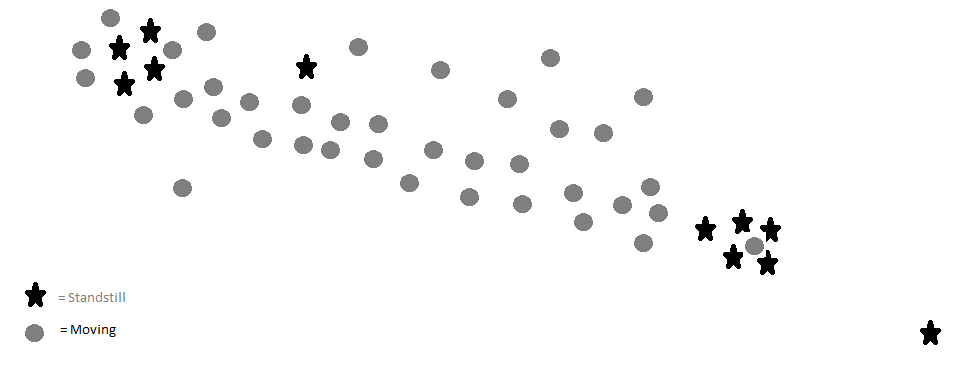
\includegraphics[scale=0.5]{graphics/pointtype-example}
	\end{center}
\end{frame}	
\begin{frame}
\frametitle{Noise}
	\begin{center}
		%Make example picture with noise points.
		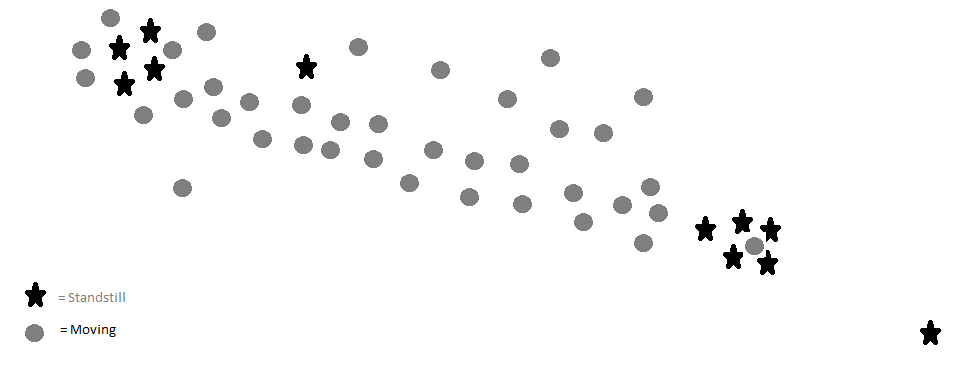
\includegraphics[scale=0.5]{graphics/pointtype-example}
	\end{center}
\end{frame}	

\subsubsection{DBSCAN} %Partial Clustering? - from presentation notes.
\begin{frame}
\frametitle{Expected data}
	\begin{itemize}
		\item Partitional - No need for hierarchies.
		\item Exclusive - Separated clusters.
		\item Partial - Need for expected outliers.
		\item Density based - The number of data points is important.
	\end{itemize}
\end{frame}	
\begin{frame}
\frametitle{DBSCAN Parameters}
	\begin{itemize}
		\item Core points
		\item Border points
		\item Noise points
	\end{itemize}
\end{frame}	

%Slide med de 2 parameter og hvordan vi sætter dem. Hvad de betyder etc.

\subsection{Reduction strategies}
\subsubsection{Other reduction strategies}
\begin{frame}
\frametitle{Reduction strategy - Rectangle}
\begin{multicols}{2}
	\begin{itemize}
		\item Advantages:
		\begin{itemize}
			\item Property ...
		\end{itemize}
		\item Disadvantages:
		\begin{itemize}
			\item Property ...
		\end{itemize}
	\end{itemize}
\columnbreak
	\begin{center}
		%Images of Convex Hull vs Square
		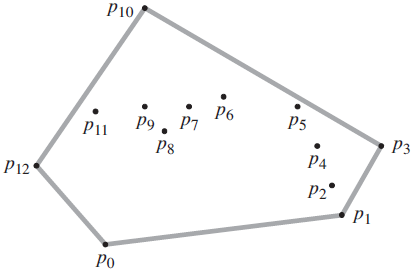
\includegraphics[scale=0.5]{graphics/convexHull-example}\\
		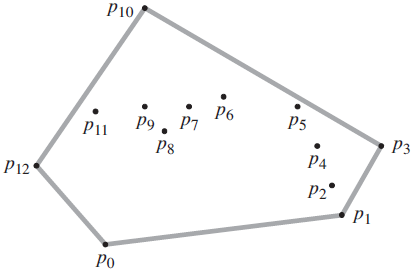
\includegraphics[scale=0.5]{graphics/convexHull-example}
	\end{center}
\end{multicols}
\end{frame}
\begin{frame}
\frametitle{Reduction strategy - Elipse}
\begin{multicols}{2}
	\begin{itemize}
		\item Advantages:
		\begin{itemize}
			\item Property ...
		\end{itemize}
		\item Disadvantages:
		\begin{itemize}
			\item Property ...
		\end{itemize}
	\end{itemize}
\columnbreak
	\begin{center}
		%Images of Convex Hull vs Circle
		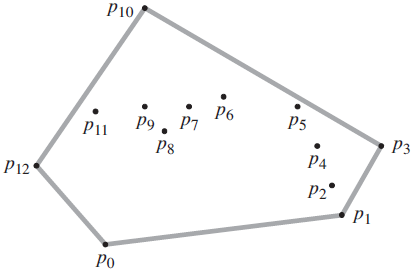
\includegraphics[scale=0.5]{graphics/convexHull-example}\\
		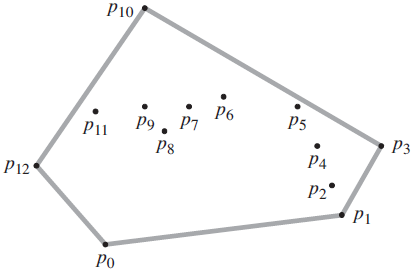
\includegraphics[scale=0.5]{graphics/convexHull-example}
	\end{center}
\end{multicols}
\end{frame}	
\begin{frame}
\frametitle{Reduction strategy - Polygon}
\begin{multicols}{2}
	\begin{itemize}
		\item Advantages:
		\begin{itemize}
			\item Property ...
		\end{itemize}
		\item Disadvantages:
		\begin{itemize}
			\item Property ...
		\end{itemize}
	\end{itemize}
\columnbreak
	\begin{center}
		%Images of Convex Hull vs Polygon
		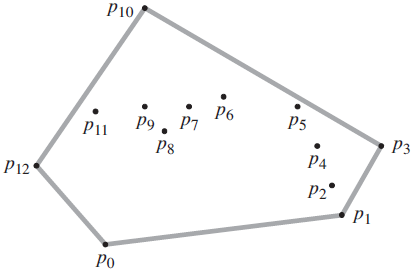
\includegraphics[scale=0.5]{graphics/convexHull-example}\\
		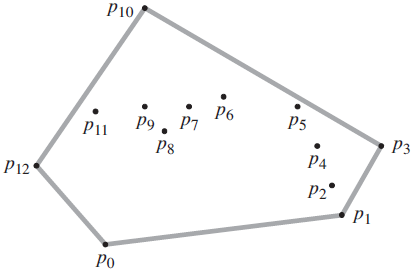
\includegraphics[scale=0.5]{graphics/convexHull-example}
	\end{center}
\end{multicols}
\end{frame}
\begin{frame}
\frametitle{Reduction strategy - Convex Hull}
\begin{multicols}{2}
	\begin{itemize}
		\item Advantages:
		\begin{itemize}
			\item Property ...
		\end{itemize}
		\item Disadvantages:
		\begin{itemize}
			\item Property ...
		\end{itemize}
	\end{itemize}
\columnbreak
	\begin{center}
		%Images of Convex Hull vs Polygon
		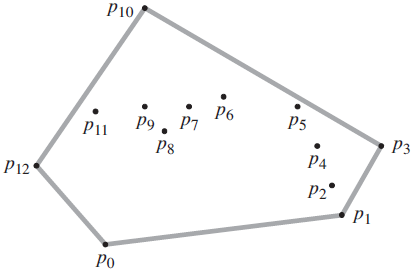
\includegraphics[scale=0.5]{graphics/convexHull-example}\\
		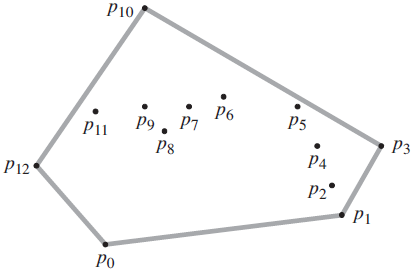
\includegraphics[scale=0.5]{graphics/convexHull-example}
	\end{center}
\end{multicols}
\end{frame}